% !TEX program = xelatex
\documentclass[12pt,a4paper,fontset=fandol]{ctexart}
\usepackage[left=22mm,right=22mm,top=22mm,bottom=22mm]{geometry}
\usepackage{amsmath,amssymb,bm,mathtools}
\usepackage{graphicx,xcolor,booktabs,longtable,array,calc}
\usepackage{tikz}
\usetikzlibrary{arrows.meta,calc,decorations.pathmorphing}
\usepackage{setspace,enumitem,fancyhdr}
\usepackage[unicode,hidelinks]{hyperref}
\setstretch{1.24}
\setlength{\parindent}{2em}
\setlength{\parskip}{.35em}
\setlength{\emergencystretch}{2em}
\setlist{nosep,leftmargin=2em}
\setcounter{secnumdepth}{-1}
\ctexset{section={format=\Large\bfseries,beforeskip=1em,afterskip=.7em},
subsection={format=\large\bfseries,beforeskip=.8em,afterskip=.4em},
subsubsection={format=\normalsize\bfseries,beforeskip=.7em,afterskip=.3em}}
\allowdisplaybreaks[2]
\tikzset{arr/.style={-{Stealth[length=2mm]},semithick},
dot/.style={circle,fill,inner sep=1.5pt}}
\providecommand{\tightlist}{\setlength{\itemsep}{0pt}\setlength{\parskip}{0pt}}
\providecommand{\pandocbounded}[1]{#1}
\newsavebox{\diagrambox}
\pagestyle{fancy}
\fancyhf{}
\renewcommand{\headrulewidth}{0pt}
\fancyfoot[C]{\small \thepage}
\setlength{\headheight}{16pt}
\begin{document}
\begin{titlepage}
\thispagestyle{empty}
\vspace*{27mm}
\begin{center}
{\LARGE\bfseries 第41届全国中学生物理竞赛\par}
\vspace{8mm}
{\LARGE\bfseries 复赛理论试题\par}
\vspace{17mm}
{\Large 试题版\par}
\end{center}
\vfill
\end{titlepage}
\setcounter{page}{1}
本卷共7题，总分320分。考试时间：9:00---12:00。所有需要评阅的解答均须写在答题纸上。

\section{第 1
题　高层建筑的摆式减振器（45分）}\label{ux7b2c-1-ux9898-ux9ad8ux5c42ux5efaux7b51ux7684ux6446ux5f0fux51cfux632fux566845ux5206}

高层建筑在风的作用下会发生晃动。在特定条件下，晃动幅度会变得较大。

（1）为减小晃动，在建筑物上安装摆式减振器。摆的悬点固定在大楼上，摆锤质量为
\(m\)，刚性摆臂长为 \(l\)，摆臂质量可忽略。大楼视为质量为 \(M\)
的刚体，其水平回复力等效为劲度系数为 \(k\) 的弹簧；整个系统总质量为
\(M+m\)。风的水平强迫力向左为正，随时间变化为

\[F(t)=H\cos\omega t,\]

其中 \(H\)、\(\omega\) 为常量，重力加速度为
\(g\)。本问只考虑摆和振子的微小振动。

\begin{center}
\begin{minipage}{\linewidth}
\centering\begingroup
\sbox{\diagrambox}{\small

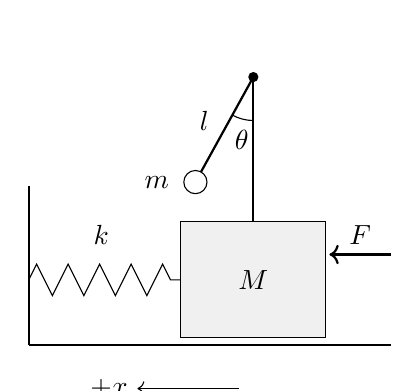
\begin{tikzpicture}[scale=.92]
\draw[thick](-3,-1.2)--(2,-1.2);
\draw[thick](-3,-1.2)--(-3,1);
\draw[decorate,decoration={zigzag,segment length=4mm,amplitude=2mm}](-3,-.3)--(-.9,-.3);
\node[above]at(-2,.05){$k$};
\draw[fill=gray!12](-.9,-1.1)rectangle(1.1,.5);
\node at(.1,-.3){$M$};
\draw[thick](.1,.5)--(.1,2.5);
\fill(.1,2.5)circle(2pt);
\draw[dashed](.1,2.5)--(.1,.8);
\draw[thick](.1,2.5)--(-.7,1.05);
\filldraw[fill=white](-.7,1.05)circle(.16)node[left=6pt]{$m$};
\node[left]at(-.38,1.9){$l$};
\draw(.1,1.9)arc(-90:-119:.6);
\node at(-.06,1.63){$\theta$};
\draw[->,thick](2,.05)--(1.15,.05)node[midway,above]{$F$};
\draw[->](-.1,-1.8)--(-1.5,-1.8)node[left]{$+x$};
\end{tikzpicture}
}
\ifdim\wd\diagrambox>.88\linewidth
\sbox{\diagrambox}{\resizebox{.88\linewidth}{!}{\usebox{\diagrambox}}}
\fi
\ifdim\ht\diagrambox>.40\textheight
\resizebox{!}{.40\textheight}{\usebox{\diagrambox}}
\else\usebox{\diagrambox}\fi
\par\smallskip{\small 建筑物与摆式减振器；位移和摆角向左为正\par}
\endgroup\end{minipage}
\end{center}

（1.1）求大楼在强迫力作用下产生的稳定振动的振幅。

（1.2）指出没有减振器时，什么风频率使大楼受迫振幅最大；针对此频率，减振器满足什么条件才能最大限度减小大楼的受迫振动？

（2）风频率为第（1.2）问所得频率的 \(\sqrt{0.99}\)
倍。求没有减振器时大楼的受迫振幅。若摆长 \(l\)
满足第（1.2）问的条件，要使振幅降到无减振器时的 \(1\%\)，求 \(m/M\)。

（3）实际装置将摆锤浸没在固定于大楼的油池中。油的质量可忽略，或已包含在
\(M\) 中。油相对大楼静止，摆锤相对油的速度为 \(\boldsymbol v'\)
时受到阻力 \(\boldsymbol f=-\gamma\boldsymbol v'\)，\(\gamma\)
为常量。写出含阻尼力的系统运动方程组，列式时不作小振幅近似，无需求解。定性说明阻尼力为何不可缺少。

\clearpage

\section{第 2
题　台球碰撞、滑动与30°经验规则（50分）}\label{ux7b2c-2-ux9898-ux53f0ux7403ux78b0ux649eux6ed1ux52a8ux4e0e30ux7ecfux9a8cux89c4ux521950ux5206}

台球 \(Q\) 撞击静止的目标球 \(T\)。两球质量均为 \(m\)、半径均为
\(R\)，质量分布均匀。碰撞前 \(Q\) 球质心速度为
\(\boldsymbol v_0=v_0\boldsymbol e_y\)，转动角速度为
\(\boldsymbol\omega_0\)。碰撞时间极短，两球之间没有摩擦，碰撞完全弹性；球与桌面为点接触。取桌面内右手直角坐标系，\(z\)
轴竖直向上，\(x\) 向右，\(y\) 为入射方向。

\begin{center}
\begin{minipage}{\linewidth}
\centering\begingroup
\sbox{\diagrambox}{\small
\scalebox{.85}{
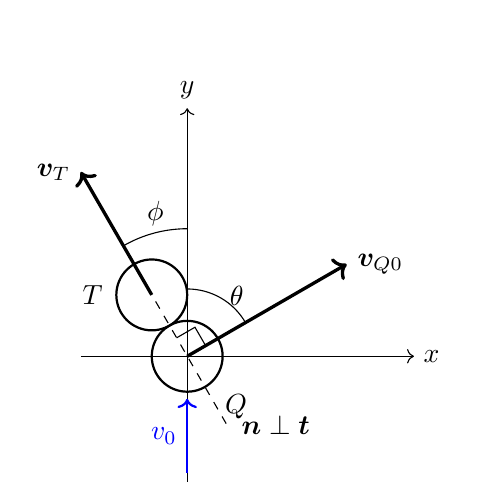
\begin{tikzpicture}[scale=.9]
\draw[->](-1.5,0)--(3.2,0)node[right]{$x$};
\draw[->](0,-2)--(0,3.5)node[above]{$y$};
\draw[thick](0,0)circle(.5)node[below right=10pt]{$Q$};
\draw[thick](-.5,.866)circle(.5)node[left=14pt]{$T$};
\draw[dashed](-1.5,2.6)--(.55,-.95);
\draw[->,very thick](-.5,.866)--(-1.5,2.598)node[left]{$\boldsymbol v_T$};
\draw[->,very thick](0,0)--(2.25,1.30)node[right]{$\boldsymbol v_{Q0}$};
\draw[->,blue,thick](0,-1.65)--(0,-.6)node[left,midway]{$v_0$};
\draw(0,1.8)arc(90:120:1.8);\node at(-.45,2.02){$\phi$};
\draw(0,.95)arc(90:30:.95);\node at(.7,.85){$\theta$};
\draw(-.15,.2598)--(.1098,.4098)--(.2598,.15);
\node[below]at(1.25,-.7){$\boldsymbol n\perp\boldsymbol t$};
\end{tikzpicture}
}
}
\ifdim\wd\diagrambox>.88\linewidth
\sbox{\diagrambox}{\resizebox{.88\linewidth}{!}{\usebox{\diagrambox}}}
\fi
\ifdim\ht\diagrambox>.40\textheight
\resizebox{!}{.40\textheight}{\usebox{\diagrambox}}
\else\usebox{\diagrambox}\fi
\par\smallskip{\small 等质量台球碰撞；角度均相对入射方向标记\par}
\endgroup\end{minipage}
\end{center}

（1）碰撞后瞬间，\(T\) 球和 \(Q\) 球的运动方向与 \(y\) 轴的夹角分别为
\(\phi\)、\(\theta\)，如图。求两球运动方向夹角，以及 \(Q\) 球的质心速度
\(\boldsymbol v_Q\) 和转动角速度 \(\boldsymbol\omega\)，用
\(\phi,v_0,\boldsymbol\omega_0\) 等表示。

（2）碰撞后，\(Q\) 球在桌面摩擦力作用下经过 \(\Delta t\)
才达到无滑滚动。已知动摩擦系数 \(\mu\)、重力加速度 \(g\)，以及
\(\phi,v_0,\omega_{0x},\omega_{0y}\)。用这些量及 \(m,R\) 表示下列结果：

（2.1）碰撞后的任意时刻，球上与桌面接触的点称为该时刻的 \(C\)
点。求碰撞后瞬间该点对桌面的速度 \(\boldsymbol v_{C0}\) 的 \(x,y\)
分量。

（2.2）求达到纯滚的时间 \(\Delta t\)。

（2.3）以碰撞后瞬间球心位置为桌面内原点，求纯滚前球心轨迹
\(x(t),y(t)\)。

（2.4）定性指出纯滚后球心轨迹形状，并给出最终速度与 \(y\) 轴夹角
\(\theta_f\) 的正切。

\clearpage

（3）击球者在开球时给静止 \(Q\) 球一个沿 \(+y\) 的水平冲量
\(\mathcal J\)。作用点在过球心的竖直大圆面内，距桌面高度为
\(h\)。求使球立即无滑滚动的特定 \(h\)。

\begin{center}
\begin{minipage}{\linewidth}
\centering\begingroup
\sbox{\diagrambox}{\small
\scalebox{.85}{
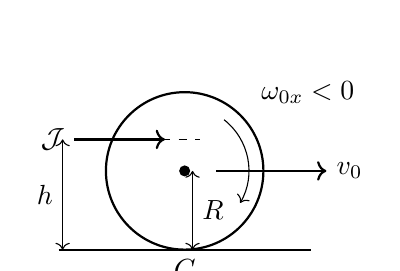
\begin{tikzpicture}
\draw[thick](-1.6,0)--(1.6,0);
\draw[thick](0,1)circle(1);\fill(0,1)circle(2pt);
\draw[->,thick](-1.4,1.4)--(-.25,1.4);
\node[left]at(-1.4,1.4){$\mathcal J$};
\draw[dashed](-.92,1.4)--(.2,1.4);
\draw[<->](-1.55,0)--(-1.55,1.4)node[midway,left]{$h$};
\draw[<->](.1,0)--(.1,1)node[midway,right]{$R$};
\draw[->,thick](.4,1)--(1.8,1)node[right]{$v_0$};
\draw[->](.5,1.65)arc(52:-30:.82);
\node[right]at(.85,2){$\omega_{0x}<0$};
\node[below]at(0,0){$C$};
\end{tikzpicture}
}
}
\ifdim\wd\diagrambox>.88\linewidth
\sbox{\diagrambox}{\resizebox{.88\linewidth}{!}{\usebox{\diagrambox}}}
\fi
\ifdim\ht\diagrambox>.40\textheight
\resizebox{!}{.40\textheight}{\usebox{\diagrambox}}
\else\usebox{\diagrambox}\fi
\par\smallskip{\small 水平冲量的作用高度与球心位置\par}
\endgroup\end{minipage}
\end{center}

（4）探讨台球手熟悉的30°经验规则。在第（3）问选定高度的条件下，\(Q\)
球以纯滚状态撞击 \(T\) 球，\(T\) 球沿角度 \(\phi\) 飞出。

（4.1）求碰撞后至纯滚前球心的 \(x(t),y(t)\)。

（4.2）求最终夹角 \(\theta_f\) 的正切。

（4.3）\(\theta_f\) 在 \(\phi=\phi_m\) 处取极大值
\(\theta_{fm}\)。求它们，并计算
\(\phi_m\pm5^\circ\)、\(\phi_m\pm10^\circ\) 时的
\(\theta_f\)，完成下表。

{\def\LTcaptype{table} % do not increment counter
\begin{longtable}[]{@{}
  >{\raggedright\arraybackslash}p{(\linewidth - 10\tabcolsep) * \real{0.1667}}
  >{\raggedright\arraybackslash}p{(\linewidth - 10\tabcolsep) * \real{0.1667}}
  >{\raggedright\arraybackslash}p{(\linewidth - 10\tabcolsep) * \real{0.1667}}
  >{\raggedright\arraybackslash}p{(\linewidth - 10\tabcolsep) * \real{0.1667}}
  >{\raggedright\arraybackslash}p{(\linewidth - 10\tabcolsep) * \real{0.1667}}
  >{\raggedright\arraybackslash}p{(\linewidth - 10\tabcolsep) * \real{0.1667}}@{}}
\toprule\noalign{}
\begin{minipage}[b]{\linewidth}\raggedright
\(\phi\)
\end{minipage} & \begin{minipage}[b]{\linewidth}\raggedright
\(\phi_m=\)
\end{minipage} & \begin{minipage}[b]{\linewidth}\raggedright
\(\phi_m+5^\circ\)
\end{minipage} & \begin{minipage}[b]{\linewidth}\raggedright
\(\phi_m+10^\circ\)
\end{minipage} & \begin{minipage}[b]{\linewidth}\raggedright
\(\phi_m-5^\circ\)
\end{minipage} & \begin{minipage}[b]{\linewidth}\raggedright
\(\phi_m-10^\circ\)
\end{minipage} \\
\midrule\noalign{}
\endhead
\bottomrule\noalign{}
\endlastfoot
\(\theta_f\) & & & & & \\
\end{longtable}
}

\clearpage

\section{第 3
题　注水温度与表面张力的微观模型（45分）}\label{ux7b2c-3-ux9898-ux6ce8ux6c34ux6e29ux5ea6ux4e0eux8868ux9762ux5f20ux529bux7684ux5faeux89c2ux6a21ux578b45ux5206}

液体与其他介质（包括其蒸气）的分界面称为液体表面，表面张力系数是表征液体性质的重要特征量。

（1）某油井内未抽出的石油为油气混合物，温度为
\(100^\circ\mathrm C\)。其密度是混有表面活性物质的水（下称``水''）的
\(80\%\)，比热容是这种水的
\(60\%\)。记这一状态为参考状态。石油和水的混合物表面张力系数与温度、压强近似满足

\[\frac\sigma{10^{-3}\,\mathrm{N/m}}
=60+0.065\frac T{\mathrm K}
-24.0\frac p{\mathrm{bar}}
+3.15\frac{p^2}{\mathrm{bar}^2}.\]

混合物的等体压强系数为常量

\[\beta=7.28\times10^{-3}\,\mathrm{bar/K}.\]

参考状态下混合物的压强与绝对温度成正比，比例系数为
\(\beta\)。某固定岩层区域中原来的石油都处于参考状态，抽出其一半，同时注入等体积的水，使区域内混合物总体积始终不变。未抽出的石油与注入水均匀混合，混合物体积等于两种液体体积之和。抽油较快，抽出的石油与注入的水之间的热交换可以忽略。求为了使区域内最终混合物的表面张力系数最小，注入水应取的摄氏温度。

\begin{center}
\begin{minipage}{\linewidth}
\centering\begingroup
\sbox{\diagrambox}{\small

\begin{tikzpicture}
\draw[thick](0,0)rectangle(2.5,2.8);
\fill[orange!20](.02,.02)rectangle(2.48,1.4);
\fill[blue!15](.02,1.4)rectangle(2.48,2.78);
\draw[dashed](0,1.4)--(2.5,1.4);
\node at(1.25,.75){剩余石油 $V$};\node at(1.25,2.05){注入水 $V$};
\draw[->,thick](-1.2,2.2)--(-.1,2.2)node[midway,above]{$t_w$};
\draw[->,thick](2.6,2.2)--(4,2.2)node[midway,above]{抽出油 $V$};
\node[below]at(1.25,0){区域总体积 $2V$ 不变};
\begin{scope}[xshift=5.2cm]
\draw[thick](0,0)rectangle(2.5,2.8);\fill[green!15](.02,.02)rectangle(2.48,2.78);
\node at(1.25,1.8){均匀混合};\node at(1.25,1.1){末态 $T_f,\ p_f$};
\node[below]at(1.25,0){体积相等，热容量不同};
\end{scope}
\end{tikzpicture}
}
\ifdim\wd\diagrambox>.88\linewidth
\sbox{\diagrambox}{\resizebox{.88\linewidth}{!}{\usebox{\diagrambox}}}
\fi
\ifdim\ht\diagrambox>.40\textheight
\resizebox{!}{.40\textheight}{\usebox{\diagrambox}}
\else\usebox{\diagrambox}\fi
\par\smallskip{\small 等体抽油注水与混合热量交换\par}
\endgroup\end{minipage}
\end{center}

（2）假设表面张力全部归结为表面层粒子与内部粒子的邻近粒子数不同，而两者粒子间距相同。表面层每粒子的邻近粒子数是内部的
\(\zeta\) 倍，\(0<\zeta<1\)。液体摩尔质量为 \(\mu\)、摩尔汽化热为
\(L_m\)、质量密度为 \(\rho\)，阿伏加德罗常量为
\(N_A\)。导出这个模型中表面张力系数 \(\sigma\) 的表达式。

\clearpage

\section{第 4
题　质子层析与量子散射尺度（45分）}\label{ux7b2c-4-ux9898-ux8d28ux5b50ux5c42ux6790ux4e0eux91cfux5b50ux6563ux5c04ux5c3aux5ea645ux5206}

（1）质子半径约为
\(0.850\,\mathrm{fm}\)，其内部包含带电荷和不带电荷的粒子。希望用电子对质子内部电荷分布进行200层断层扫描，估算被加速电子所需的动能，用
\(\mathrm{GeV}\)
表示。计算狭义相对论与极端相对论结果的差别是否小于狭义相对论结果的
\(1\%\)。本问不计电磁相互作用的影响。

（2）静止质量为 \(m\)、电荷为 \(Z_1e\) 的粒子向电荷为 \(Z_2e\)
的固定靶散射。当两者中心间距为 \(r\)、入射粒子动量大小为 \(p\)
时，求系统总能量。若入射粒子和靶均为质子，且两粒子中心间距的测量不确定度等于它们的中心间距，估算入射质子的速度
\(v\)。假设中心间距测量的不确定度与入射粒子位置测量的不确定度近似相等。本问按非相对论处理。

已知

\[e=1.60\times10^{-19}\,\mathrm C,
\qquad m_e=9.11\times10^{-31}\,\mathrm{kg},\]

\[h=6.63\times10^{-34}\,\mathrm{kg\,m^2/s},
\qquad c=3.00\times10^8\,\mathrm{m/s},\]

\[\varepsilon_0=8.85\times10^{-12}\,\mathrm{C^2/(N\,m^2)}.\]

\clearpage

\section{第 5
题　四导线磁阱与蒸发冷却（45分）}\label{ux7b2c-5-ux9898-ux56dbux5bfcux7ebfux78c1ux9631ux4e0eux84b8ux53d1ux51b7ux537445ux5206}

实现稀薄原子气体的玻色---爱因斯坦凝聚，需要磁阱囚禁和降温等技术。本题研究一种四导线磁阱的近轴磁场和势能。

（1）四根相互平行的无限长直导线，横截面可忽略，垂直穿过边长为 \(a,b\)
的长方形四个顶点。电流大小均为 \(I\)，方向如下图：左上、右下电流沿
\(+z\)，右上、左下沿 \(-z\)。以长方形中心为原点，取 \(x\) 轴垂直于长为
\(b\) 的边，\(y\) 轴垂直于长为 \(a\) 的边，建立右手直角坐标系。点
\(P=(x,y,0)\) 在原点附近，\(|x|\ll a\)、\(|y|\ll b\)，\(a,b\)
为同阶量。求 \(O,P\) 两点磁感应强度，并将可作近似的结果保留到领头阶。

\begin{center}
\begin{minipage}{\linewidth}
\centering\begingroup
\sbox{\diagrambox}{\small

\begin{tikzpicture}
\draw[dashed](-2,-1.5)rectangle(2,1.5);
\draw[->](-2.7,0)--(3.1,0)node[right]{$x$};\draw[->](0,-2)--(0,2.3)node[above]{$y$};
\node[below left]at(0,0){$O$};\fill(.55,.55)circle(2pt)node[right]{$P(x,y)$};
\foreach \x/\y/\sign in {-2/1.5/+,-2/-1.5/-,2/1.5/-,2/-1.5/+}{
\draw[fill=white,thick](\x,\y)circle(.13);
\if\sign+\fill(\x,\y)circle(1.5pt);\else\draw(\x-.08,\y-.08)--(\x+.08,\y+.08);\draw(\x-.08,\y+.08)--(\x+.08,\y-.08);\fi}
\draw[<->](-2,-2.4)--(2,-2.4)node[midway,below]{$a$};
\draw[<->](2.5,-1.5)--(2.5,1.5);\node[right]at(2.5,.55){$b$};
\node[above left]at(-2,1.5){$+I$};\node[below left]at(-2,-1.5){$-I$};
\node[above right]at(2,1.5){$-I$};\node[below right]at(2,-1.5){$+I$};
\end{tikzpicture}
}
\ifdim\wd\diagrambox>.88\linewidth
\sbox{\diagrambox}{\resizebox{.88\linewidth}{!}{\usebox{\diagrambox}}}
\fi
\ifdim\ht\diagrambox>.40\textheight
\resizebox{!}{.40\textheight}{\usebox{\diagrambox}}
\else\usebox{\diagrambox}\fi
\par\smallskip{\small 四导线位置与电流方向；圆点出纸面，叉号入纸面\par}
\endgroup\end{minipage}
\end{center}

（2）原子固有磁矩为
\(\boldsymbol S\)。将磁矩视为形状、电流不随旋转改变的微小电流圈，证明它在磁场
\(\boldsymbol B\) 中的势能为

\[W_m=-\boldsymbol S\cdot\boldsymbol B.\]

（3）把原子限制在 \(x-y\)
平面原点附近，并通过实验手段使磁矩方向始终与当地磁场相反。求其受力，保留到领头阶。

（4）一团原子被囚禁在柱形区域内，横截面平行于 \(x-y\) 平面、半径为
\(R_1\)，\(R_1\ll a,b\)；柱高远小于
\(R_1\)，原子密度近似均匀，磁矩均与当地磁场相反。以 \(O\)
为势能零点，求平均势能。缓慢蒸发一部分原子，使余下原子团向中心收缩为半径
\(R_1/5\)、高度不变的圆柱，密度保持不变。求冷却后的总原子数、总势能和平均势能。已知真空磁导率为
\(\mu_0\)。

\clearpage

\section{第 6
题　引力散射与星光偏折（45分）}\label{ux7b2c-6-ux9898-ux5f15ux529bux6563ux5c04ux4e0eux661fux5149ux504fux629845ux5206}

广义相对论预言星光经过太阳附近会发生偏折，1919年的日全食观测曾检验这一效应。本题先在牛顿理论下计算，再用弱场有效折射率模型计算。

（1）在牛顿动力学和万有引力框架下，质量为 \(m\) 的质点在原点处质量
\(M\gg m\) 的引力场中运动。平面极坐标轨道为

\[r(\theta)=\frac p{1+e\cos\theta},\qquad-\pi<\theta\le\pi,\]

其中半通径 \(p>0\)、偏心率 \(e\ge0\)。若 \(e>1\)，存在 \(\theta_{\max}\)
使 \(-\theta_{\max}<\theta<\theta_{\max}\)。求 \(\theta_{\max}\)
及其取值范围。

（2）由质点的机械能 \(E\) 和相对于原点的轨道角动量大小 \(L\)，导出
\(p(E,L)\)、\(e(E,L)\)。

（3）一个物体以速度 \(v_0\) 从外太空飞入太阳系，瞄准距离为
\(b\)，即初始速度所在直线到太阳中心的距离。设
\(v_0^2b/(GM_\odot)\gg1\)。求飞出方向相对原入射方向的偏折角
\(\Delta\varphi\)：

（i）入射物是陨石；

（ii）入射物是一束星光，恰好掠过太阳表面进入观测站，此时可近似取
\(b=R_\odot\)。

\begin{center}
\begin{minipage}{\linewidth}
\centering\begingroup
\sbox{\diagrambox}{\small

\begin{tikzpicture}
\draw[dashed](-3,0)--(4,0);\fill(0,0)circle(3pt)node[below]{太阳};
\draw[dashed](-3,1.3)--(1.7,1.3);
\draw[->,blue,thick](-3,1.3)--(-1.9,1.3)node[midway,above]{$v_0$};
\draw[thick](-1.9,1.3)..controls(-.7,1.3)and(.6,1.2)..(1.45,.94)--(3.8,.10);
\draw[->,thick](2.4,.6)--(3.1,.35);
\draw[<->](-1.1,0)--(-1.1,1.3)node[midway,left]{$b$};
\draw[dashed](1.45,.94)--(3.8,.94);
\draw(2.5,.94)arc(0:-20:1.05);\node[right]at(2.65,.74){$\Delta\varphi$};
\end{tikzpicture}
}
\ifdim\wd\diagrambox>.88\linewidth
\sbox{\diagrambox}{\resizebox{.88\linewidth}{!}{\usebox{\diagrambox}}}
\fi
\ifdim\ht\diagrambox>.40\textheight
\resizebox{!}{.40\textheight}{\usebox{\diagrambox}}
\else\usebox{\diagrambox}\fi
\par\smallskip{\small 远处入射方向、瞄准距离和出射偏折角\par}
\endgroup\end{minipage}
\end{center}

（4）弱场广义相对论效应可用等效相对折射率

\[n_{\rm eff}(r)=1-\frac{2\varphi(r)}{c^2}\]

表示，其中 \(\varphi(r)\) 是牛顿引力势。光线满足费马原理
\(\delta\int_A^B n_{\rm eff}(r)dl=0\)。若 \(n_{\rm eff}\) 与 \(\theta\)
无关，以 \(\theta=\theta(r)\) 写轨迹，有

\[\frac d{dr}\left(
\frac{r^2\theta'}{\sqrt{1+r^2\theta'^2}}n_{\rm eff}(r)
\right)=0,\qquad\theta'=\frac{d\theta}{dr}.\]

用这一关系重新计算掠过太阳表面的星光偏折角。已知太阳质量
\(M_\odot\)、太阳半径 \(R_\odot\)、引力常量 \(G\) 和光速 \(c\)。

\clearpage

\section{第 7
题　圆环电子、磁通周期与配对模型（45分）}\label{ux7b2c-7-ux9898-ux5706ux73afux7535ux5b50ux78c1ux901aux5468ux671fux4e0eux914dux5bf9ux6a21ux578b45ux5206}

超导环中磁通量的量子化单位为
\(h/(2e)\)。为理解这一现象，考虑一维圆环上非相对论、无相互作用电子的稳定运动。电子质量为
\(m\)，圆环半径为 \(R\)，环上状态的波函数为

\[\psi(x)=\exp\left(\frac i\hbar px\right),\]

其中 \(x=R\theta\) 标记环上的位置，\(p\)
为电子动量，\(h=2\pi\hbar\)，电子电荷为 \(-e\)，\(e>0\)。

\begin{center}
\begin{minipage}{\linewidth}
\centering\begingroup
\sbox{\diagrambox}{\small

\begin{tikzpicture}
\draw[thick](0,0)ellipse(2 and .8);\fill(-1.2,-.64)circle(3pt)node[below]{电子};
\draw[dashed](0,0)--(1.5,.53)node[midway,above]{$R$};
\draw[->,very thick](0,-1.2)--(0,1.8)node[above]{$\Phi$};
\draw[->](1.45,-.55)arc(-30:45:1.65 and .65);
\node[right]at(2,.3){正向绕环};
\node[below]at(.7,-1.5){$x=R\theta$};
\end{tikzpicture}
}
\ifdim\wd\diagrambox>.88\linewidth
\sbox{\diagrambox}{\resizebox{.88\linewidth}{!}{\usebox{\diagrambox}}}
\fi
\ifdim\ht\diagrambox>.40\textheight
\resizebox{!}{.40\textheight}{\usebox{\diagrambox}}
\else\usebox{\diagrambox}\fi
\par\smallskip{\small 一维圆环的角坐标与正向磁通\par}
\endgroup\end{minipage}
\end{center}

（1）由波函数的单值性，给出电子动量 \(p\) 所有可能取值。

（2）环内通入轴对称、垂直环面的磁通量
\(\Phi\)，箭头方向为磁通正向。本题把 \(\Phi\) 视为连续变量。电子动量变为
\(p'=p+eA\)，\(A\) 是沿环切向的磁矢势大小，能量为
\(E=p'^2/(2m)\)。给出单电子能量 \(E\) 与磁通量的关系。

（3）环上有 \(N\)
个无相互作用电子，在接近绝对零度时满足：任意两个电子具有不同动量，系统总能量最小。证明系统最低总能量
\(E_{\rm tot}\) 随 \(\Phi\) 周期变化，并给出周期。

（4）在 \(-h/(2e)\le\Phi\le h/(2e)\) 内，求平均能量
\(\overline E=E_{\rm tot}/N\) 的变化关系。指出：\(N\) 为奇数时
\(\Phi=0\) 的平均能量小于 \(|\Phi|=h/(2e)\) 时；\(N\) 为偶数时相反。

（5）在一个配对模型中，动量为 \(p'\) 和 \(-p'\)
的电子必须同时存在或同时不存在。考虑半径同为 \(R\)、电子总数为 \(2N\)
的两个圆环，电子可以在两环任意分配。

（5.1）证明两环各带奇数电子时，电子数相差最小且 \(\Phi=0\)
时平均能量最低；两环各带偶数电子时，电子数相差最小且 \(\Phi=h/(2e)\)
时平均能量最低。分别记这两个极小情形为a、b，并证明其动量占据满足上述配对条件。

（5.2）比较a、b两种情形：a为两环各有 \(N=2M+1\)
个电子，\(\Phi=0\)；b为两环有 \(N_1=2(M+1)\)、\(N_2=2M\)
个电子，\(\Phi=h/(2e)\)。其中 \(M\)
为正整数。证明电子平均能量之比在电子数趋于无穷时趋于一。

\end{document}
